% DO NOT COMPILE THIS FILE DIRECTLY!
% This is included by the other .tex files.
\begin{frame}
  \frametitle{Upcoming Supercomputers}
    \begin{center}
      
\includegraphics[width=.25\textwidth]{./figures/ecp} \\
      % \includegraphics[width=.75\textwidth]{./figures/go} 
    \end{center}
  \begin{columns}[T]
    \begin{column}{0.49\textwidth}
      \begin{center}
        {\bf Aurora}\\
        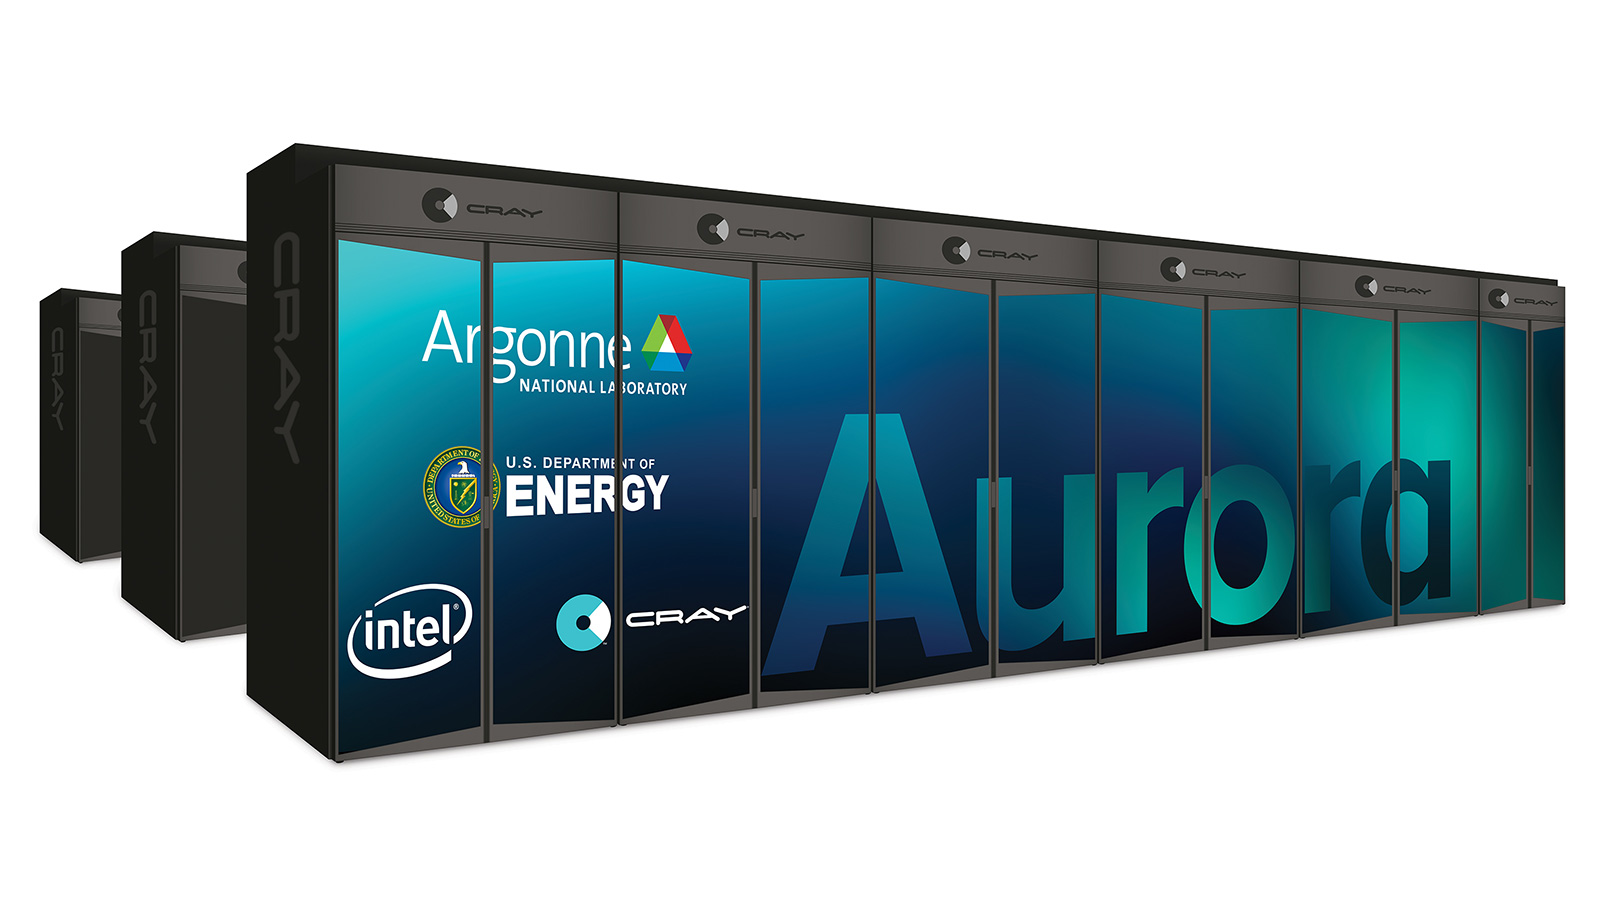
\includegraphics[width=0.75\textwidth]{./figures/aurora}
      \end{center}
    \end{column}
    \begin{column}{0.49\textwidth}
      \begin{center}
        {\bf Frontier}\\
        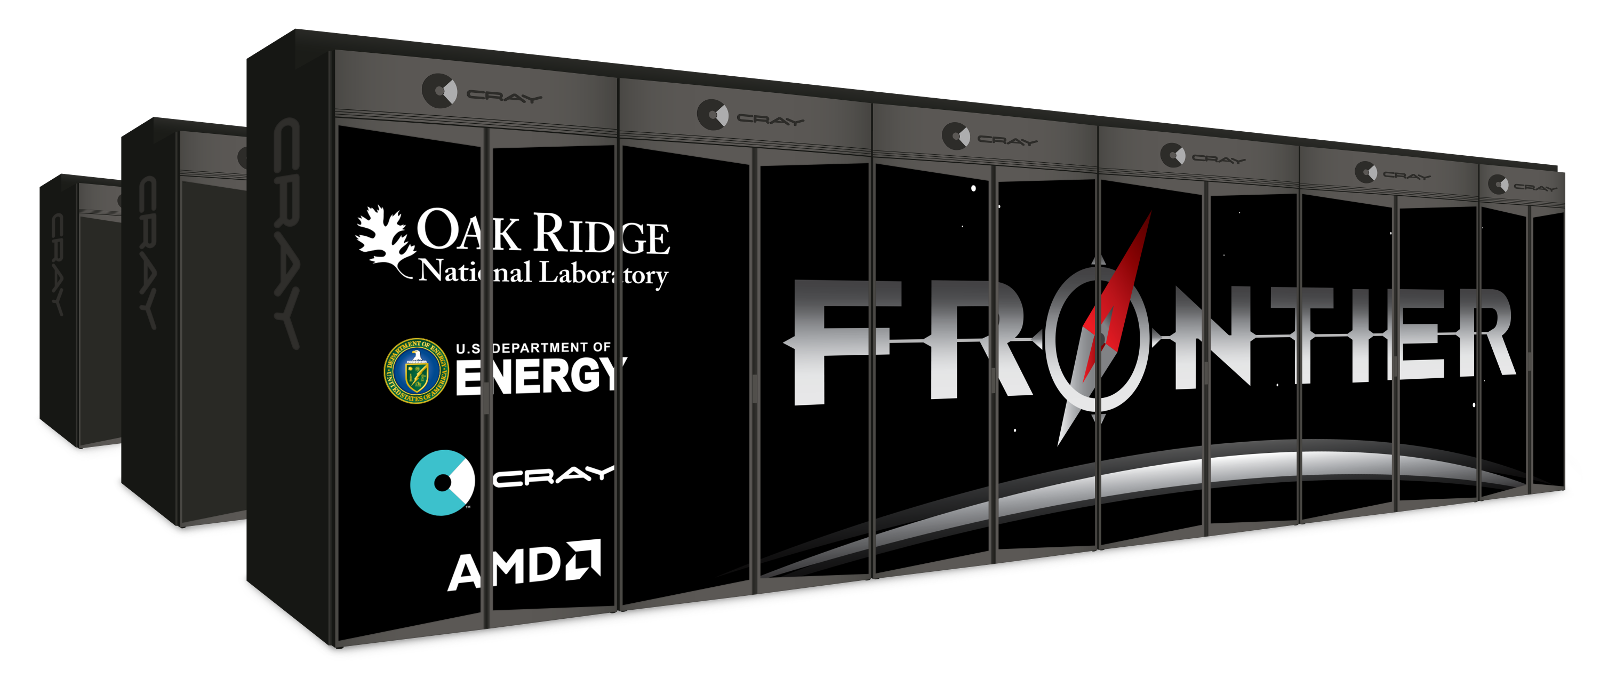
\includegraphics[width=0.75\textwidth]{./figures/frontier}
      \end{center}
    \end{column}
  \end{columns}
  \begin{columns}[T]
    \begin{column}{0.49\textwidth}
    \begin{itemize}
      \item Intel’s Xe compute architecture.
      \item $>$ 1 exaflops
    \end{itemize}
    \end{column}
    \begin{column}{0.49\textwidth}
      \begin{itemize}
        \item AMD EPYC processors and Radeon Instinct GPU
        \item 1.5 exaflops
      \end{itemize}
    \end{column}
  \end{columns}
\end{frame}

\begin{frame}
  \frametitle{Power System}
  \begin{columns}
    \begin{column}{0.45\textwidth}
      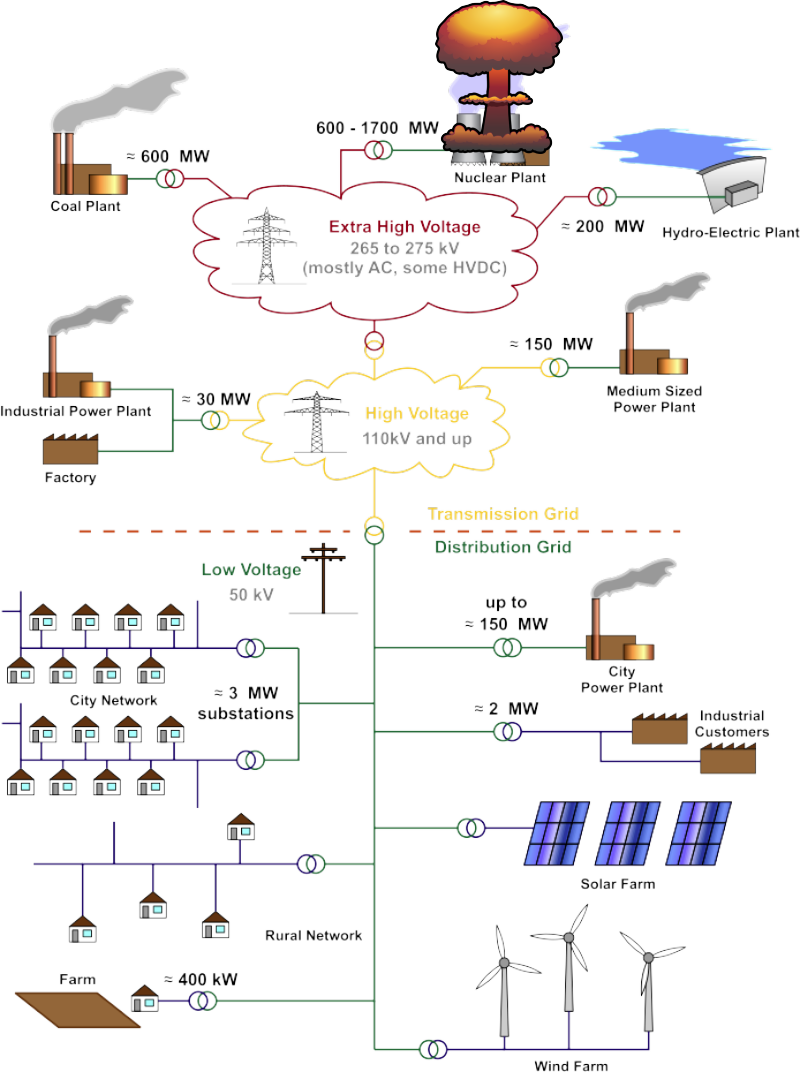
\includegraphics[width=\textwidth]{figures/slides.png}
    \end{column}
    \begin{column}{0.45\textwidth}
      \begin{center}
        % \includegraphics[width=0.8\textwidth]{figures/DampedSine.png}
      \end{center}
      \begin{itemize}
        \item Protect against contingency scenarios
        \item Demand is uncertain
        \item Generation is uncertain (solar, wind, water)
        \item Recent developments in renewable energies lead to less mass in generators decreasing inertia
        \item Less inertia worsens effects of uncertainty
      \end{itemize}
    \end{column}
  \end{columns}
\end{frame}

\begin{frame}
  \frametitle{Complex Networks}
  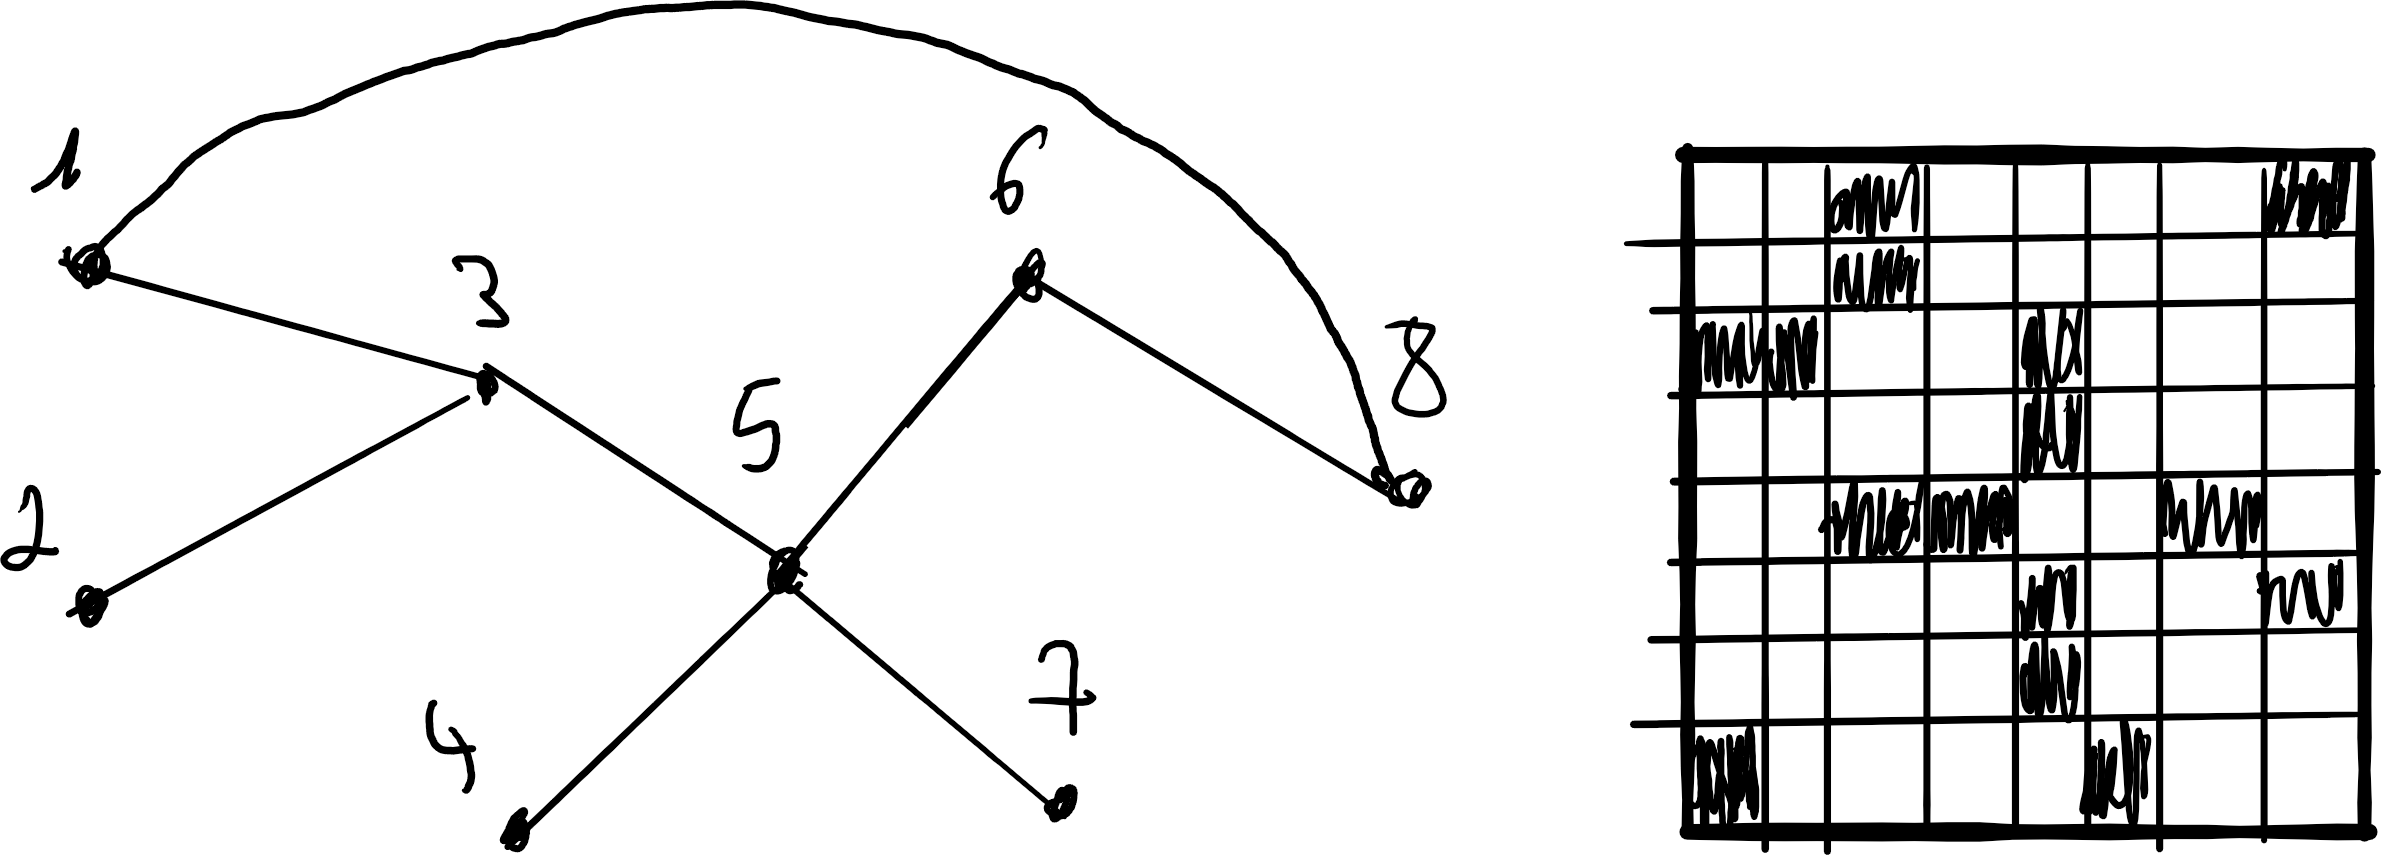
\includegraphics[width=\textwidth]{figures/complexn}
  \begin{itemize}
    \item Examples: traffic, Internet, pipelines, power grid
    \item Connection pattern is irregular but not random
  \end{itemize}
\end{frame}

\begin{frame}[fragile]
  \frametitle{NLP: Alternate Current Optimal Power Flow}
  \begin{itemize}
    \item {\bf Objective}
    \begin{itemize}
      \item Generation $P_g$ and its cost $c$ at generators $g_i$:
      $ \minimize \sum^G_{i=1} c_i(P_{g_i})$, where $c_i$ is the cost of generator $g_i$
    \end{itemize}
    \item {\bf Constraints}
    \begin{itemize}
      \item Kirchhoff's law: What flows in must flow out (nonlinear, non-convex in ACOPF)
      \begin{align*}
        V_k e^{-j\theta_k} & \sum^{N}_{m=0} (G_{km} + jB_{km})V_m e^{j\theta_m} = P_k - j Q_k,\ k = 1, \dots, N \\
        \text{where}\\
        V_k &\text{ voltage magnitude at node } k\\
        \theta &\text{ voltage angle at node } k\\
        G_{km} + jB_{km}& \text{ element of nodal admittance matrix}\\
        P_k , Q_k &\text{ net real and reactive power entering and leaving node } k
      \end{align*}
      \item Line limits defined through voltage angles $\theta$ at the buses $m$ and $n$:
      $$ \theta^{min}_{nm} \leq \theta_n - \theta_m \leq \theta^{max}_{nm}$$
    \end{itemize}
  \end{itemize}
\end{frame}

\begin{frame}[fragile]
  \frametitle{Use Interior-Point for NLP}
  {\bf Solve}
  \begin{align*}
  &\minimize f(x)\\ 
  \text{with}&\\
  &g(x) \geq 0, \ i=1,\dots, m \\
  &c(x) = 0, \ j=1,\dots, l \\
  \end{align*}
  {\bf using Newton and barrier functions}
  \begin{align*}
  &\minimize \phi_\mu := f(x) - \mu \sum^m_{i=1} \ln g(x)\\ 
  \text{with}&\\
  &c(x) = 0, \ j=1,\dots, l 
  \end{align*}
  \begin{itemize}
    \item Barrier functions exacerbate ill-conditioning
  \end{itemize}
\end{frame}

\begin{frame}[fragile]
  \frametitle{Interior-Point and GPUs}
  {\bf Current State}
  \begin{itemize}
    \item De facto standard solver: Ipopt
    \item Very ill-conditioned system (up $1e^{16}$)
    \item Requires indefinite sparse direct inertia revealing solver
    \item Ipopt only supports direct solver (exception: Pardiso)
    \item default MUMPS, preferred are HSL libary MA27, MA57 
    \item PIPS-NLP \footnote{\cite{pips}} \footnote{https://github.com/Argonne-National-Laboratory/PIPS} implements Schur complement for two-stage optimization
    \item HiOp\footnote{https://github.com/LLNL/hiop} mixed dense-sparse solver 
  \end{itemize}
\end{frame}
\begin{frame}
  \frametitle{Distributed Parallel Interior-Point Solvers}
  \begin{center}
    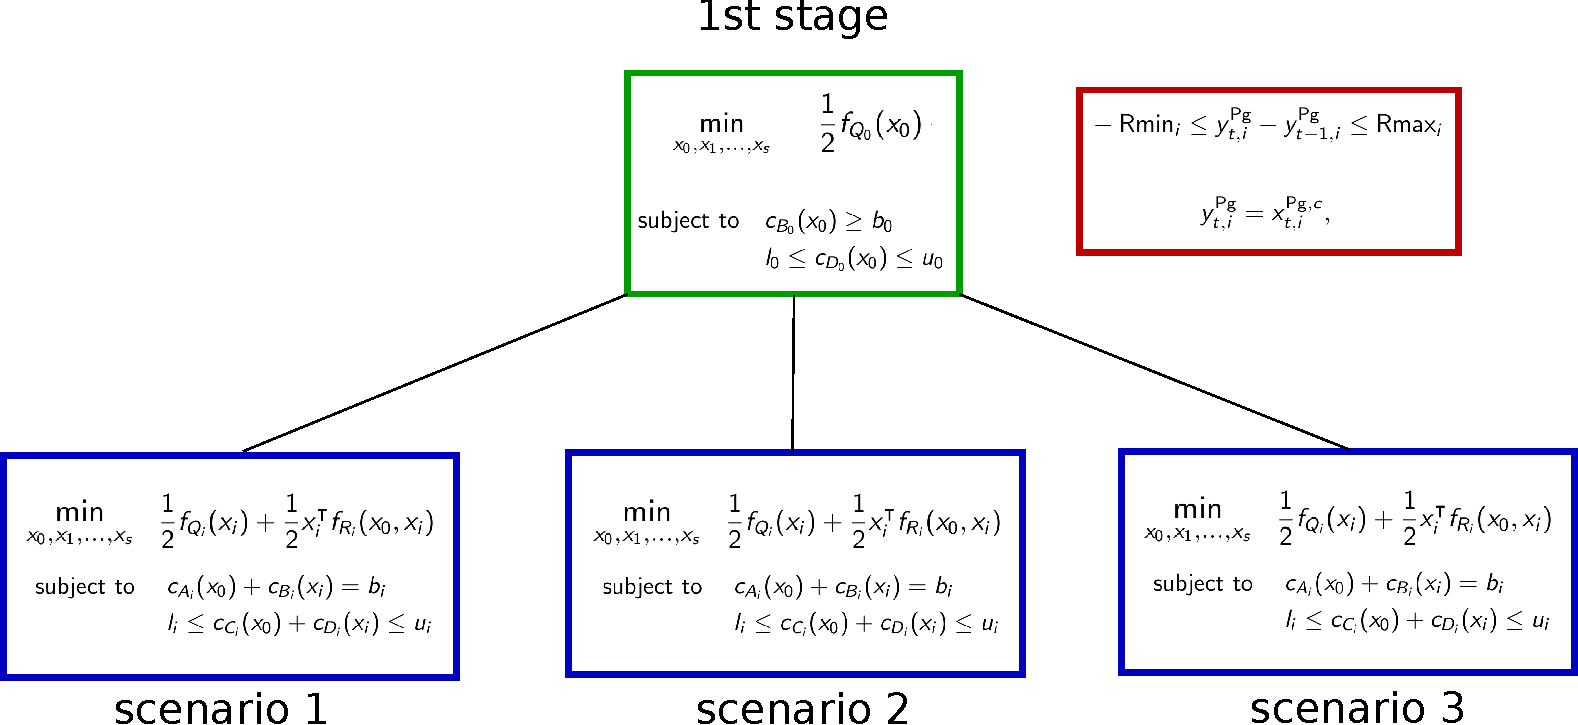
\includegraphics[width=0.65\textwidth]{figures/twostageopt}
  \end{center}
  \begin{columns}[T]
    \begin{column}{0.45\textwidth}
      {\bf PIPS-NLP}
      \begin{itemize}
        \item Model in \lstinline{StructJuMP.jl}
        \item Sparse algebra in PIPS
        \item JuMP currently has no GPU support
        \item Julia support for Intel and AMD GPUs
      \end{itemize}
    \end{column}
    \begin{column}{0.45\textwidth}
      {\bf HiOp}
      \begin{itemize}
        \item Mixed-dense sparse interface for subproblems
        \item Interface will have GPU support
        \item MOI interface \lstinline{Hiop.jl}
        \item Rapid prototyping Julia, production full C++
      \end{itemize}
    \end{column}
  \end{columns}

  
\end{frame}


\begin{frame}[fragile]
  \frametitle{\sout{Optimal} Power Flow}
  \begin{itemize}
    \item {\bf \sout{Objective}}
    \begin{itemize}
      \item \sout{Generation cost at generators:
      $ \minimize \sum^G_{i=1} c_i(P_{g_i})$, where $c_i$ is the cost of generator $g_i$}
    \end{itemize}
    \item {\bf Constraints}
    \begin{itemize}
      \item Kirchhoff's law: What flows in must flow out (nonlinear, non-convex in ACOPF)
      \begin{align*}
        V_k e^{-j\theta_k} & \sum^{N}_{m=0} (G_{km} + jB_{km})V_m e^{j\theta_m} = P_k - j Q_k,\ k = 1, \dots, N \\
        \text{where}\\
        V_k &\text{ voltage magnitude at node } k\\
        \theta &\text{ voltage angle at node } k\\
        G_{km} + jB_{km}& \text{ element of nodal admittance matrix}\\
        P_k , Q_k &\text{ net real and reactive power entering and leaving node } k
      \end{align*}
      \item \sout{Line limits: $ \theta^{min}_{nm} \leq \theta_n - \theta_m \leq \theta^{max}_{nm}$}
    \end{itemize}
  \end{itemize}
\end{frame}

\begin{frame}[fragile]
  \frametitle{Power Flow}
  {\bf Nonlinear equations}
  \begin{itemize}
      \item Kirchhoff's law: What flows in must flow out (nonlinear, non-convex in ACOPF)
      \begin{align*}
        V_k e^{-j\theta_k} & \sum^{N}_{m=0} (G_{km} + jB_{km})V_m e^{j\theta_m} = P - jQ,\ k = 1, \dots, N \\
        \text{where}\\
        V_k &\text{ voltage magnitude at node } k\\
        \theta &\text{ voltage angle at node } k\\
        G_{km} + jB_{km}& \text{ element of nodal admittance matrix}\\
        P, Q &\text{ net real and reactive power entering and leaving node } k
      \end{align*}
      \item Use Newton-Raphson to solve nonlinear equations
      \item Reference implementation: MATPOWER in Matlab
  \end{itemize}
\end{frame}

\begin{frame}
  \frametitle{Implementation}
  {\bf Goals}
  \begin{itemize}
    \item Compute Jacobian using automatic differentiation
    \item Implement a preconditioner
    \item Implement a Krylov method
    \item No computation on the host in main loop, no data transfer
    \item All in Julia, no external calls if possible
  \end{itemize}
\end{frame}

\begin{frame}
  \frametitle{}
  \centering
  {\Huge Automatic Differentiation}
\end{frame}

\begin{frame}[fragile]
  \frametitle{Derivatives}
  {\bf Newton-Raphson}
  \begin{minipage}{0.8\textwidth}
    \begin{lstlisting}
    go = true
    while(go)
      dx .= jacobian(x)\f(x)
      x  .= x .- dx
      go = norm(f(x)) < tol ? true : false
    end
    \end{lstlisting}
   \end{minipage}
  {\bf Automatic Differentiation}
  \begin{itemize}
    \item \lstinline{F = f(x)} $\rightarrow$ \alert{\lstinline{J = jacobian(x)}}\footnote{\cite{RevelsLubinPapamarkou2016}}
    \item Two modes: \Colorbox{green}{Adjoint} or \Colorbox{red}{tangent}
    \item \Colorbox{green}{\lstinline{adj(x, y) = (J(x))'*y)}}, \Colorbox{red}{\lstinline{tgt(x,d) = J(x)*d}} 
    \item \Colorbox{green}{\lstinline{size(x) >> size(F)}} or \Colorbox{red}{\lstinline{size(x) <= size(F)}}
    \item number of buses $\propto$ \lstinline{size(x) = size(F)}
  \end{itemize}
\end{frame}

\begin{frame}
  \frametitle{Jacobian Coloring}
  \begin{center}
    \begin{figure}
      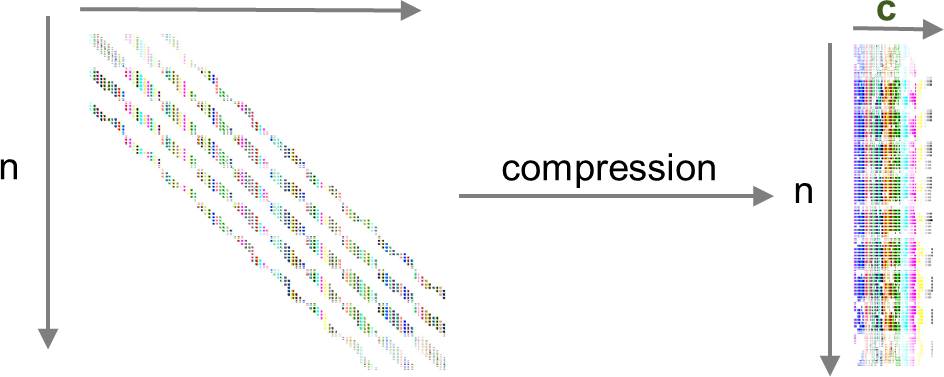
\includegraphics[width=0.65\textwidth]{figures/compression}
      \caption{Jacobian compression}
    \end{figure}
  \end{center}
  \begin{itemize}
    \item Using greedy algorithm in \lstinline{SparseDiffTools.jl}
    \item To get full Jacobian, one has to do $c$ times \lstinline{tgt(x,d) = J(x)*d}
    \item Complexity for Jacobian goes from $\bigo{n} \times cost(f)$ to $\bigo{c} \times cost(f)$
  \end{itemize}
\end{frame}

% \begin{frame}
%   \frametitle{AD on GPUs in Julia}
%   \begin{center}
%       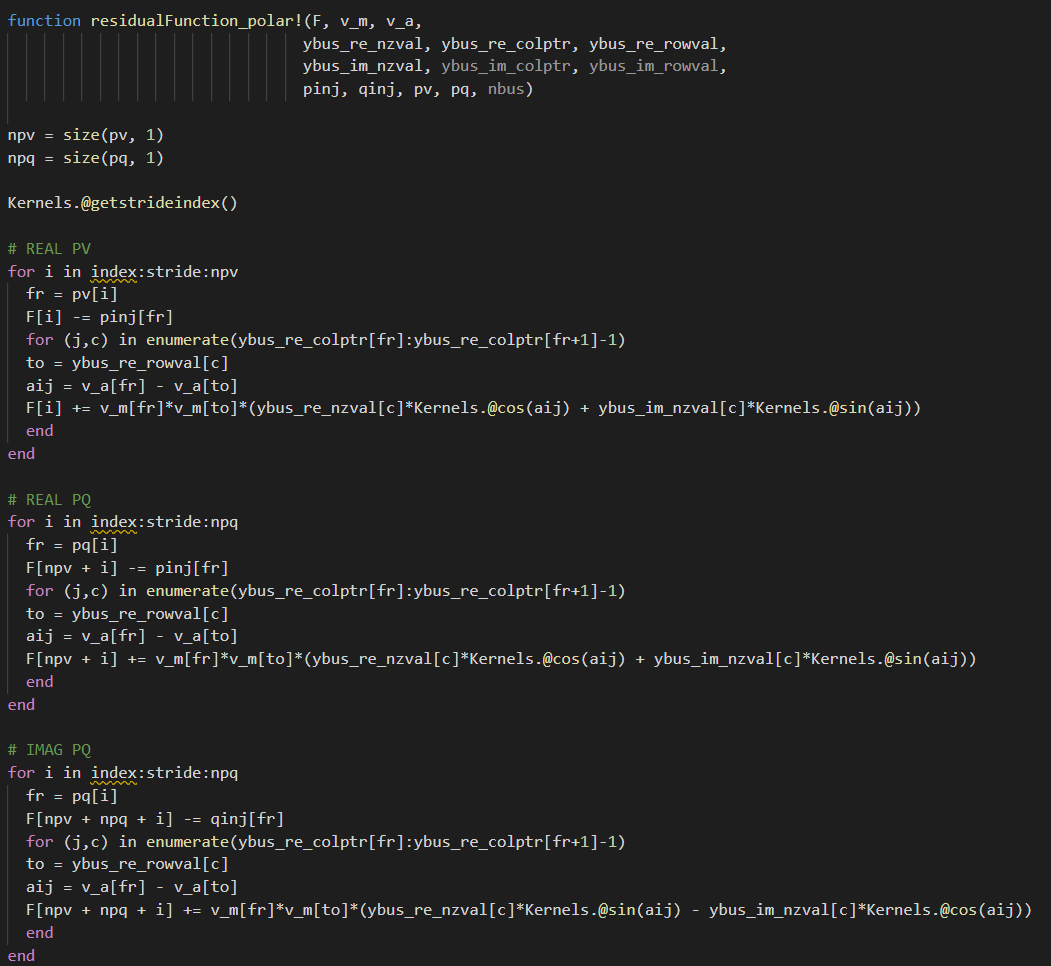
\includegraphics[width=0.75\textwidth]{figures/F}
%   \end{center}
% \end{frame}
\begin{frame}
  \frametitle{AD on GPUs in Julia}
  \begin{center}
    \lstinline{F = T(undef, n)}
  \end{center}
  \begin{itemize}
    \item Float vector: \lstinline{T = Vector\{Float64\}}
    \item Arbitrary precision vector: \lstinline{T = Vector\{BigFloat\}}
    \item First-order tangent: \lstinline{t1s\{N\} =  ForwardDiff.Dual\{Nothing,Float64, N\} where N}
    \item Second-order tangent: \lstinline{t2s\{M,N\} =  ForwardDiff.Dual\{Nothing,t1s\{N\}, M\} where M, N}
    \item First-order tangent vector: \lstinline{T = Vector\{t1s\{N\}\}}
    \item First-order tangent GPU vector: \lstinline{T = CuVector\{t1s\{N\}\}}
    \item Relying on \lstinline{CUDA.jl} \footnote{\cite{besard2018juliagpu}} \footnote{\cite{besard2019prototyping}}
    \item \alert{broadcast operator \lstinline{x .= a .* b}}
  \end{itemize}
\end{frame}

\begin{frame}
  \frametitle{AD on GPUs in Julia}
  \begin{columns}[T]
    \begin{column}{0.35\textwidth}
      \begin{center}
        \vspace{0.2cm}
        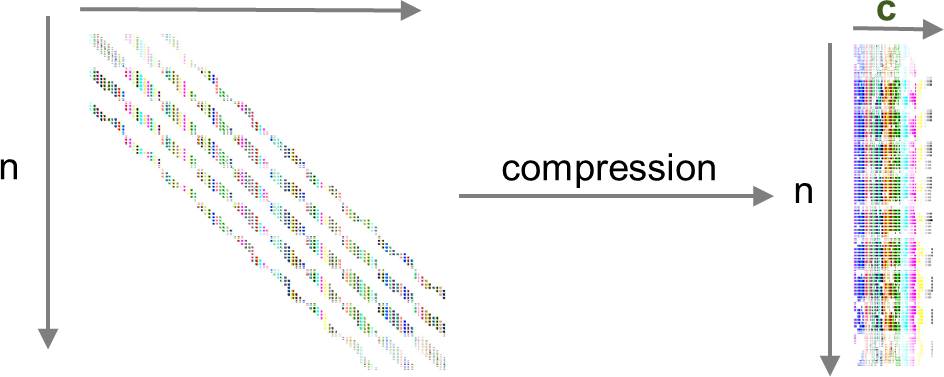
\includegraphics[width=\linewidth]{figures/compression}
      \end{center}
    \end{column}
    \begin{column}{0.6\textwidth}
      \begin{center}
        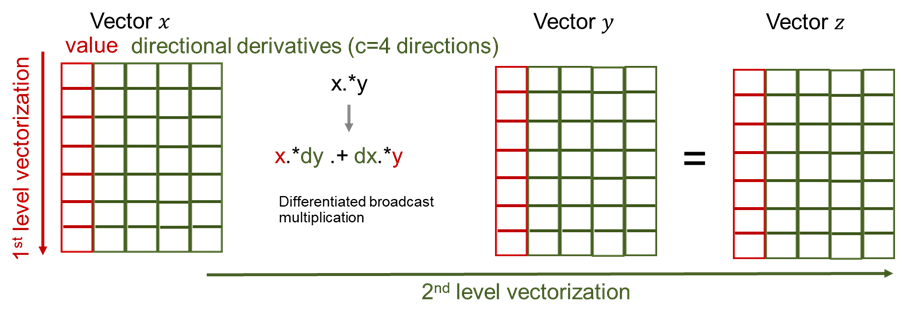
\includegraphics[width=\linewidth]{figures/simd}
      \end{center}
    \end{column}
  \end{columns}
  \begin{center}
  \end{center}
  {\bf SIMD over sparsity colors}
  \begin{itemize}
    \item Change from \lstinline{F = f(x)} to \lstinline{J = f(x)} on GPUs is a type change from \lstinline{Vector\{Float64\}} to \lstinline{CuVector\{t1s\{c\}\}}
  \end{itemize}
\end{frame}

\begin{frame}
  \frametitle{}
  \centering
  {\Huge Preconditioner}
\end{frame}

\begin{frame}
  \frametitle{Linear solver}
  {\bf Tour de Solvers, solver we have experience with}
  \begin{table}
  \begin{tabular}{p{5cm}|lll}
    MA27, MA57, MUMPS, SPQR, CUSOLVER, SPRAL SSIDS & indefinite & sparse & direct \\
    \hline
    BLAS, CUBLAS & indefinite & dense  & direct \\
    \hline
    CHOLMOD, SPRAL SSIDS& positive definite & sparse & direct \\
    \hline
    \lstinline{IterativeSolvers.jl}, \lstinline{Krylov.jl}, PETSc & indefinite & sparse & iterative \\ 
  \end{tabular}
\end{table}
  \begin{itemize}
    \item Best for GPUs: Iterative solver
    \item GMRES and BiCGSTAB \footnote{\cite{sleijpen1993bicgstab}} in \lstinline{IterativeSolvers.jl}, no GPU support 
    \item GMRES in \lstinline{Krylov.jl}, no BiCGSTAB 
    \item Wrote a naive implementation of BiCGSTAB \footnote{\cite{bicgstabVorst}}
  \end{itemize}
\end{frame}

\begin{frame}
  \frametitle{Preconditioner}
  {\bf Setup}
  \begin{itemize}
    \item Create a partitioning (METIS)
  \end{itemize}
  {\bf Update P}
  \begin{tabular}{m{0.15\textwidth}m{0.05\textwidth}m{0.3\textwidth}m{0.05\textwidth}m{0.3\textwidth}}
        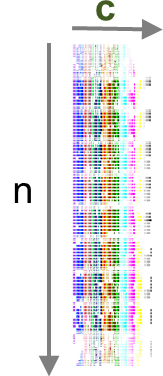
\includegraphics[width=0.15\textwidth]{./figures/compressed}
    &
    {\Huge $\rightarrow$}
    &
        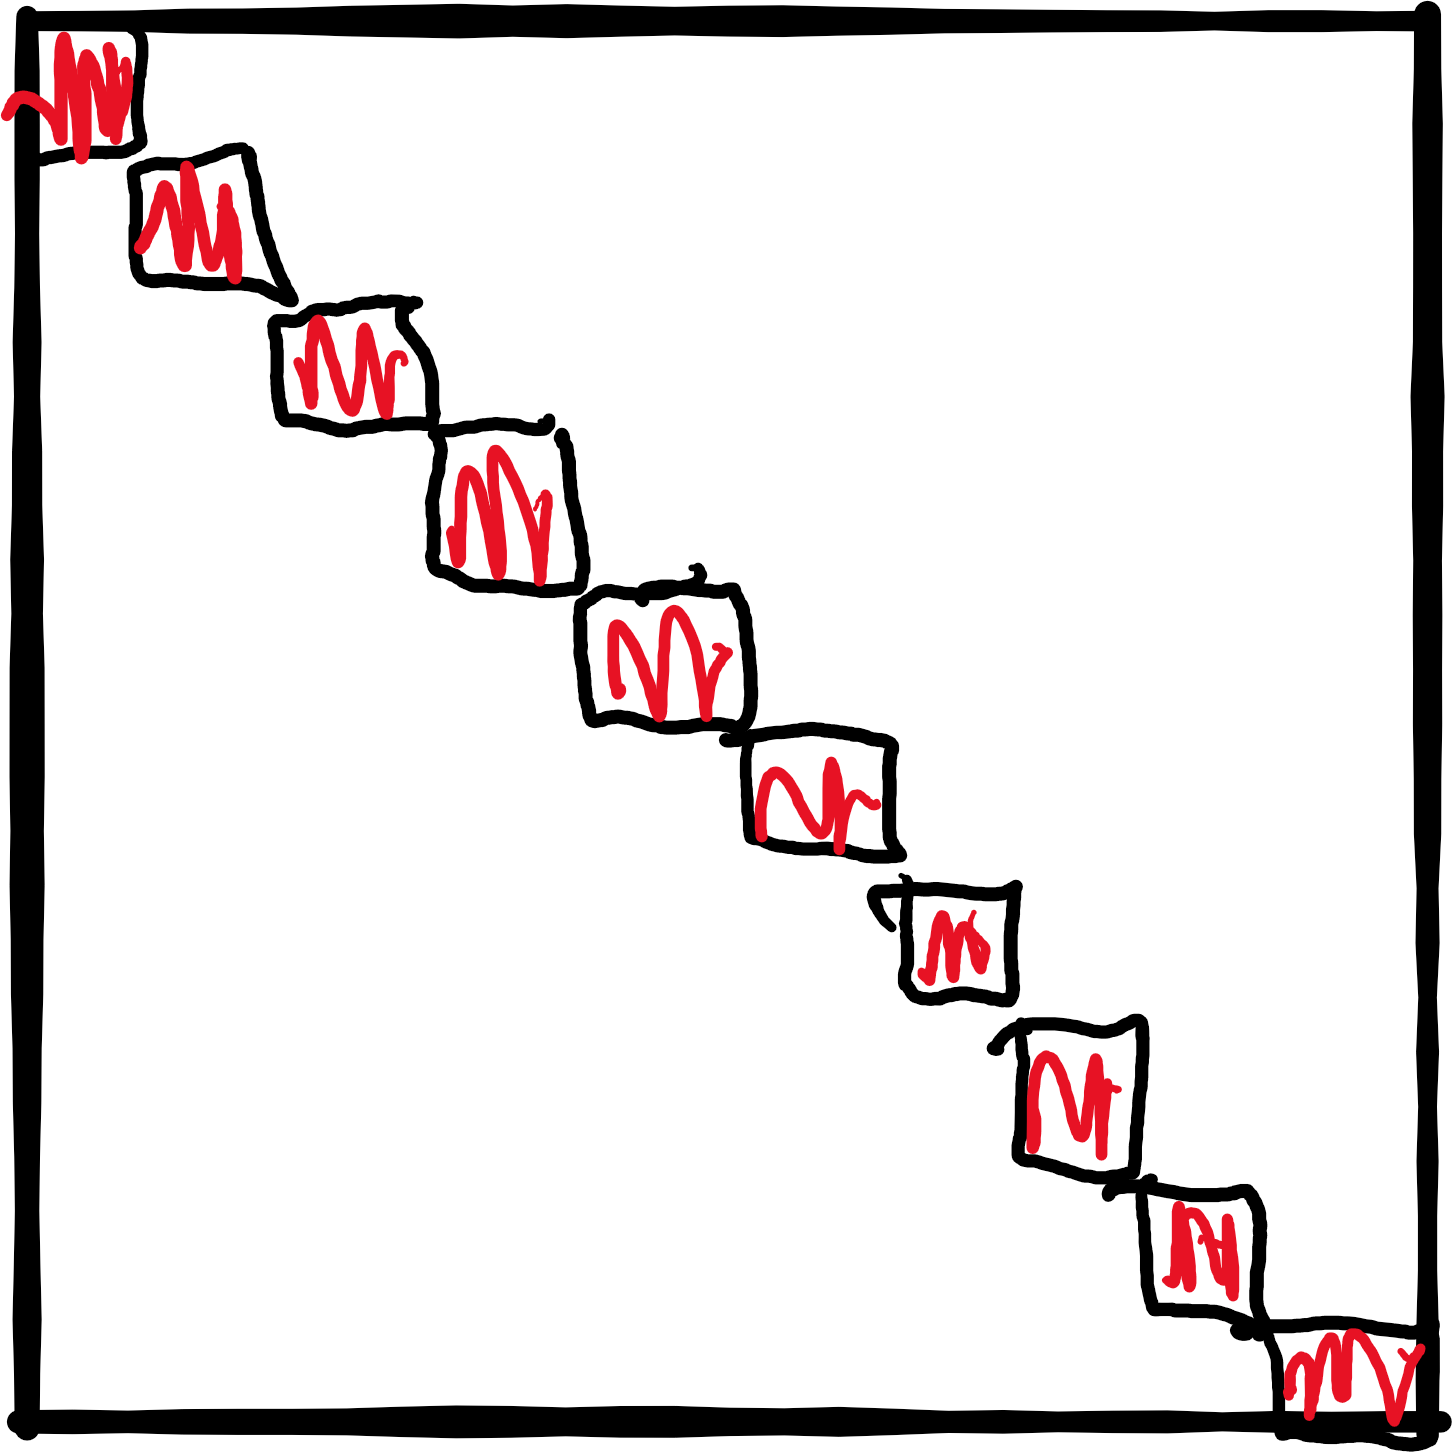
\includegraphics[width=0.3\textwidth]{figures/gpublocks}
    &
    {\Huge $\rightarrow$}
    &
        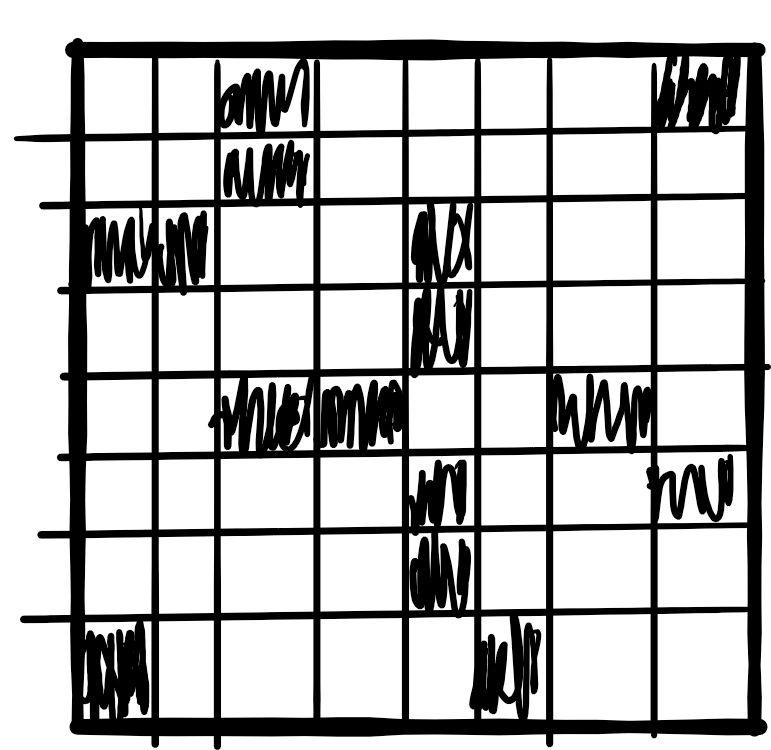
\includegraphics[width=0.3\textwidth]{./figures/csr}
    \\
  \end{tabular}
    \begin{enumerate}
      \item Read dense compressed Jacobian into dense Jacobi blocks
      \item Batch inversion of dense blocks using CUBLAS
      \item Update sparse matrix P from dense Jacobi blocks
    \end{enumerate}
  {\bf Code size}
  \begin{itemize}
    \item 200 lines of code for BOTH CPU and GPU implementation
  \end{itemize}
\end{frame}

% \begin{frame}
%   \frametitle{Preconditioner}
%   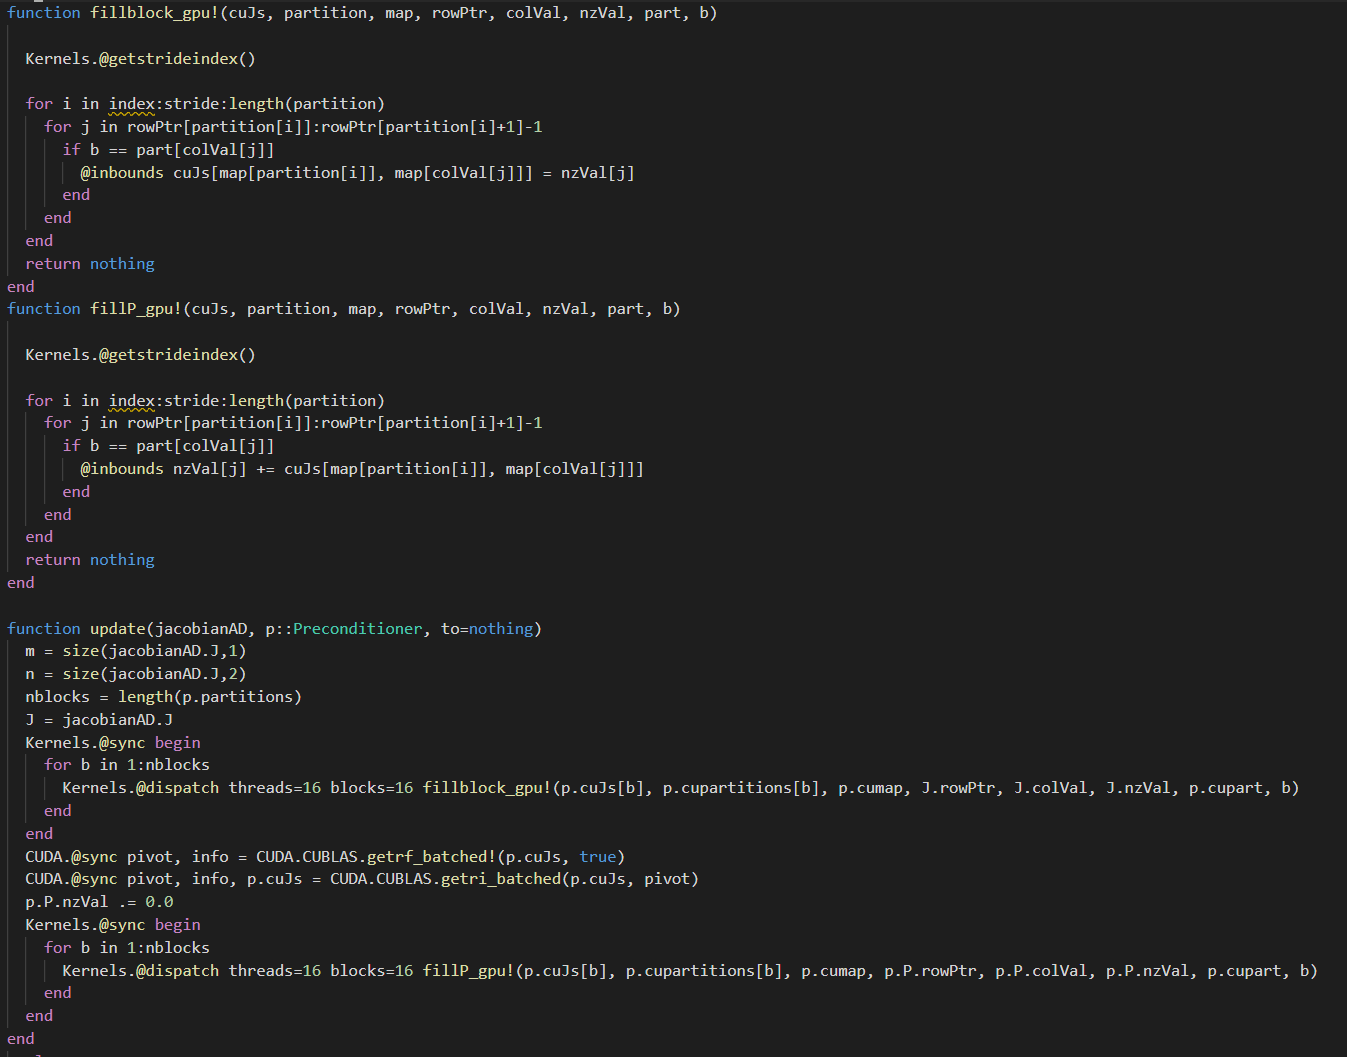
\includegraphics[width=0.95\textwidth]{figures/preconditioner}
% \end{frame}



% \begin{frame}[fragile]
%   \frametitle{Linear Solver}
%   \begin{center}
%    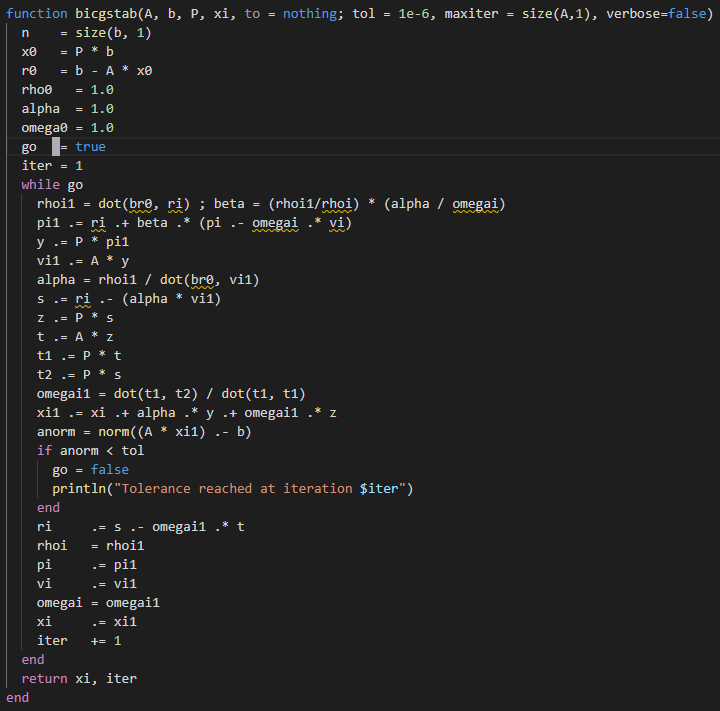
\includegraphics[width=0.7\textwidth]{figures/bicgstab.png}
%   \end{center}
% \end{frame}

% \begin{frame}
%   \frametitle{SIMD on GPUs in Julia}
%   \begin{center}
%       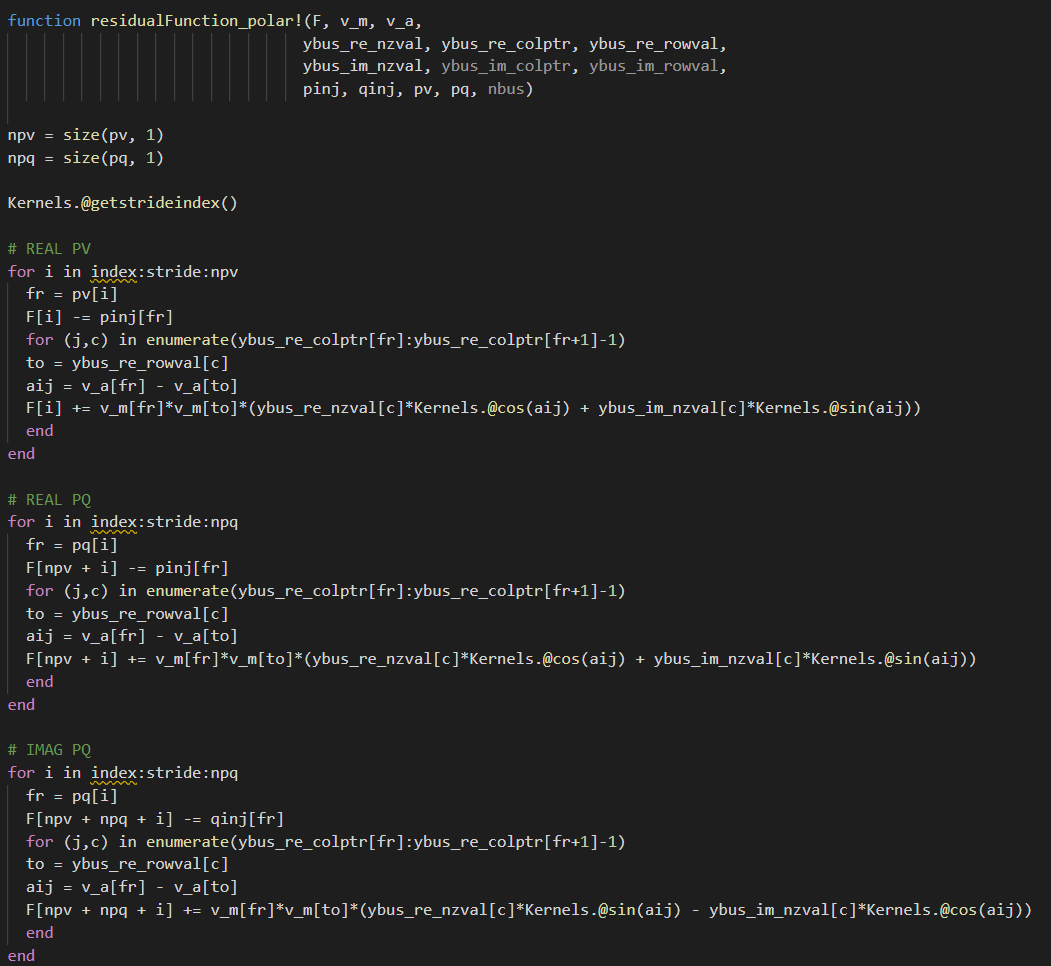
\includegraphics[width=0.75\textwidth]{figures/F}
%   \end{center}
% \end{frame}
% \begin{frame}
%   \frametitle{AD on GPUs in Julia}
%   \begin{center}
%     \lstinline{F = T(undef, n)}
%   \end{center}
%   \begin{itemize}
%     \item Float vector: \lstinline{T = Vector\{Float64\}}
%     \item Arbitrary precision vector: \lstinline{T = Vector\{BigFloat\}}
%     \item First-order tangent: \lstinline{t1s\{N\} =  ForwardDiff.Dual\{Nothing,Float64, N\} where N}
%     \item Second-order tangent: \lstinline{t2s\{M,N\} =  ForwardDiff.Dual\{Nothing,t1s\{N\}, M\} where M, N}
%     \item First-order tangent vector: \lstinline{T = Vector\{t1s\{N\}\}}
%     \item First-order tangent GPU vector: \lstinline{T = CuVector\{t1s\{N\}\}}
%     \item Relying on \lstinline{CUDA.jl} \footnote{\cite{besard2018juliagpu}} \footnote{\cite{besard2019prototyping}}
%     \item \alert{broadcast operator \lstinline{x .= a .* b}}
%   \end{itemize}
% \end{frame}

\begin{frame}
  \frametitle{}
  \centering
  {\Huge Results}
\end{frame}

\begin{frame}[fragile]
  \frametitle{ExaPF.jl}
  \begin{lstlisting}
    pkg> instantiate
    julia> target = "cuda" 
    julia> include("examples/pf.jl") 
    julia> datafile = "test/case14.raw"
    julia> sol, conv, res = pf(datafile, 8, "bicgstab") # slow
    julia> sol, conv, res = pf(datafile, 8, "bicgstab")
  \end{lstlisting}
  \begin{itemize}
    \item \url{https://exanauts.github.io/}
    \item Julia for Summit builds
    \item Other research software
    \item \url{https://github.com/exanauts/ExaPF.jl}
  \end{itemize}
\end{frame}

\begin{frame}[fragile]
  \frametitle{ExaPF.jl}
  {\bf 30,000 bus system}
  \begin{lstlisting}
    julia> datafile = "GO-Data/.../Network_30R-025/.../case.raw"
    julia> sol, conv, res = pf(datafile, 1000, "bicgstab")
  \end{lstlisting}
  \begin{itemize}
    \item \lstinline{size(J)} = 57,721 $\times$ 57,721 
    \item Block Jacobi size: 59 $\times$ 59 $\approx$ 25 MB
    \item Total GPU memory usage: 5 GB
    \item Number of Jacobian colors: 29
    \item 4 Newton iterations with $tol = 1e^{-6}$, total BiCGSTAB iterations: 3,752 
  \end{itemize}
\end{frame}

\begin{frame}
  \frametitle{Results}
  \begin{itemize}
    \item Code runs on local workstation {\it moonshot} and Summit
    \item NVIDIA Quadro GV100 based on Volta 
  \end{itemize}
\end{frame}

\begin{frame}[fragile]
  \frametitle{ExaPF.jl}
  {\bf 30,000 bus system}
  \begin{center}
   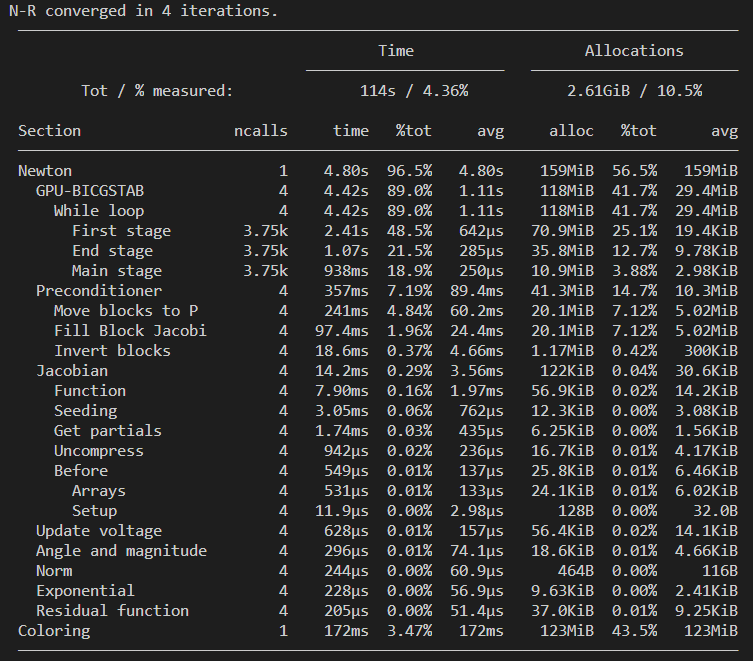
\includegraphics[width=0.8\textwidth]{figures/timings}
  \end{center}
\end{frame}

\begin{frame}
  \frametitle{Results}
  {\bf 30,000 bus system}
  \begin{itemize}
    \item CUSOLVE: 10s 
    \item Sparse Julia \lstinline{J\\F} (probably UMFPACK): 3.49s 
    \item Block Jacobi + BiCGSTAB in ExaPF.jl
    \begin{itemize}
      \item Jacobian: 14.2 ms
      \item Preconditioner: 357 ms
      \item BiCGSTAB: 4.42s
      \item Total: 4.8s
    \end{itemize}
  \end{itemize}
\end{frame}

\begin{frame}
  \frametitle{Hessian and Jacobian Coloring}
  \begin{center}
    \begin{figure}
      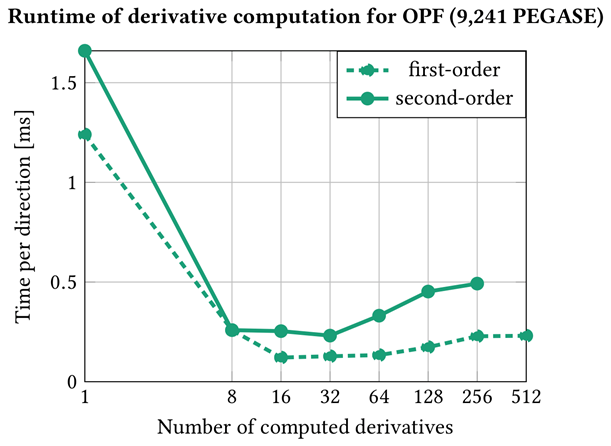
\includegraphics[width=0.45\textwidth]{figures/directionsgpu}\footnote{\cite{simdicpp}}
    \end{figure}
  \end{center}
  \begin{itemize}
    \item Number of colors for 9,241 bus system: 76, Hessian size: 580,587$\times$580,587, compressed: 580,587$\times$76
    \item GPU strategy: Effectively SIMD parallelize over colors/directions
    \item Sweet spot on NVIDIA GV100: Chunks of 32 directions (see Figure)
    \item 0.3ms per color
    \item We don’t expect number colors to exceed 500 for final case
  \end{itemize}
\end{frame}

\begin{frame}
  \frametitle{Conclusions}
  {\bf Optimization on GPUs for NLPs}
  \begin{itemize}
    \item Use ExaPF.jl in reduced gradient method for OPF
    \item Second-order optimization 
    \item Much harder systems for OPF with inequality constraints
    \item SIMD modeling framework (MOI)
    \item Support for GPU Arrays on Intel and AMD GPUs
    \item Augmented Lagrangian with domain decomposition
    \item Rapid prototyping in Julia is fast
  \end{itemize}
\end{frame}

\begin{frame}[noframenumbering,plain,allowframebreaks]{References}
    \printbibliography[heading=none]
\end{frame}



